%------------------------------------------------------------------------------
% No implementation, software engineering details, or project management
%------------------------------------------------------------------------------

%------------------------------------------------------------------------------

\begin{subsection}{The Elevator Pitch}
  Whilst advances in technology have revolutionised other industries and parts of agriculture, bringing with it radically improved methods and cost efficiencies, the way in which we identify and brand cattle is practically archaic.

  The process of marking cattle can be incredibly painful, regardless of the age of the cattle. Clearly, being subject to this pain, and the witnessing of the pain of a calf by a mother, is an point of controversy with regard to animal rights.

  Whilst branding is not said to be conducted anymore in the United Kingdom \cite{theguardian-1}

  \begin{center}
    \fbox{
      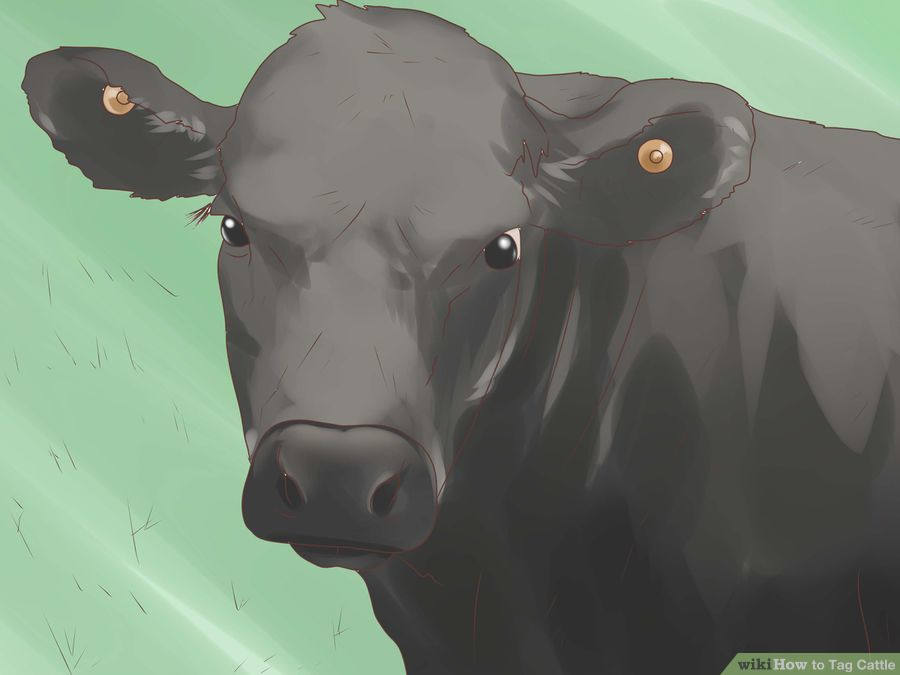
\includegraphics[width=0.5\textwidth]{images/cattle-with-ear-tag.jpg}
    }
  \end{center}
\end{subsection}

%------------------------------------------------------------------------------

\begin{subsection}{Project Description}

\end{subsection}

%------------------------------------------------------------------------------

\begin{subsection}{What is the need for the project?}

\end{subsection}
